\section{Experiments}
\subsection{Online Graph Maintenance in a Single Embedding Space}
\label{sec:single-space}

We use a controlled synthetic teacher--student task to test whether ARIAD can maintain useful neighbors while embeddings change during training, and preserve the output quality of exact top-$k$ attention with fewer similarity evaluations.

\paragraph{Setup and metrics.}
We sample $N/16$ random unit-norm centers in $\mathbb{R}^{64}$, generate 16 points per center with Gaussian jitter of standard deviation $0.10$, and normalize each point to obtain $G\in\mathbb{R}^{N\times64}$. Independently sampled Gaussian values $V\in\mathbb{R}^{N\times64}$ form the input $X=[G\mid V]\in\mathbb{R}^{N\times128}$ after per-feature standardization. The teacher uses scores $S_{ij}=(g_i^\top g_j-\mu)/\sigma$ for $j\ne i$, where $\mu$ and $\sigma$ are the global mean and standard deviation of all off-diagonal entries of $GG^\top$. Self-links are masked. For the teacher's exact top-32 set $T_i$, the target is
\begin{equation}
 y_i=\sum_{j\in T_i}
 \frac{\exp(S_{ij}/\tau)}{\sum_{\ell\in T_i}\exp(S_{i\ell}/\tau)}v_j,
 \qquad \tau=0.5.
\end{equation}
The student learns $Z=XW_z$ and $\hat V=XW_v$, both with 64 channels, using scores $z_i^\top z_j/\sqrt{64}$. Dense aggregates over all nonself nodes; Exact top-$k$ recomputes the student's exact top-32 each step; ARIAD refreshes a maintained 32-neighbor graph, initialized randomly without teacher or exact neighbors. Exact and ARIAD use the same sparse attention computation after neighbor selection. The default ARIAD search scores $C_{\mathrm{scored}}=144$ candidate slots per row: 32 retained neighbors, 80 second-order outgoing candidates, and 32 incoming-buffer candidates. This measured count includes duplicates and self-candidates before masking.

We train with full-batch Adam for 500 steps (one step per epoch), learning rate $10^{-2}$, and no weight decay, for $N\in\{1008,2000,5008,10000,20000\}$. Table~\ref{tab:single-quality} reports three paired training seeds (0, 1, 2): methods share the data, teacher, and initial student weights within each pair. Each $N$ uses one fixed dataset generated with seed 0; the three seeds vary training randomness, not datasets. MSE is evaluated after each update on the same synthetic nodes used for training, not on held-out data. \emph{Teacher match@32} is the mean fraction of $T_i$ recovered by the student's neighbors; for Dense, the top-32 of its learned scores is only a diagnostic. \emph{Current-graph recall@32} instead compares ARIAD's maintained graph with the exact top-32 under that same ARIAD student's current embeddings. Evaluation uses post-update embeddings and the graph retained from the training forward pass.

\begin{table*}[t]
\centering
\caption{Single-space output quality after 500 optimization steps ($k=32$, sparse top-32 teacher). MSE is evaluated on the training nodes; teacher match is the mean overlap fraction with the teacher top-32 set. Entries are mean $\pm$ sample standard deviation over three paired training seeds on one fixed dataset per $N$. For Dense, top-32 is extracted only for this diagnostic. ``$<$ denotes a standard deviation below display precision. The $N=1008$ runs have not fully converged. ARIAD uses $C_{\mathrm{scored}}=144$.}
\label{tab:single-quality}
\footnotesize
\setlength{\tabcolsep}{3.5pt}
\begin{tabular}{r ccc ccc}
\toprule
 & \multicolumn{3}{c}{MSE ($\times 10^{-4}$)} & \multicolumn{3}{c}{Teacher match@32} \\
\cmidrule(lr){2-4}\cmidrule(lr){5-7}
$N$ & Dense & Exact top-$k$ & ARIAD & Dense & Exact top-$k$ & ARIAD \\
\midrule
1,008 & 4.49$\pm$0.24 & 4.32$\pm$0.07 & 4.36$\pm$0.14 & 0.8155$\pm$0.0010 & 0.8079$\pm$0.0027 & 0.8031$\pm$0.0074 \\
2,000 & 5.44$\pm$0.09 & 4.79$\pm{<}$0.01 & 4.79$\pm{<}$0.01 & 0.9295$\pm$0.0002 & 0.9303$\pm{<}$0.0001 & 0.9291$\pm{<}$0.0001 \\
5,008 & 4.15$\pm$0.02 & 2.30$\pm{<}$0.01 & 2.31$\pm{<}$0.01 & 0.9554$\pm$0.0001 & 0.9583$\pm{<}$0.0001 & 0.9503$\pm$0.0001 \\
10,000 & 6.70$\pm{<}$0.01 & 1.78$\pm{<}$0.01 & 1.82$\pm{<}$0.01 & 0.9629$\pm{<}$0.0001 & 0.9686$\pm{<}$0.0001 & 0.9463$\pm$0.0003 \\
20,000 & 11.85$\pm{<}$0.01 & 0.96$\pm{<}$0.01 & 1.11$\pm{<}$0.01 & 0.9680$\pm{<}$0.0001 & 0.9767$\pm{<}$0.0001 & 0.9276$\pm$0.0002 \\
\bottomrule
\end{tabular}
\end{table*}


\begin{figure}[t]
 \centering
 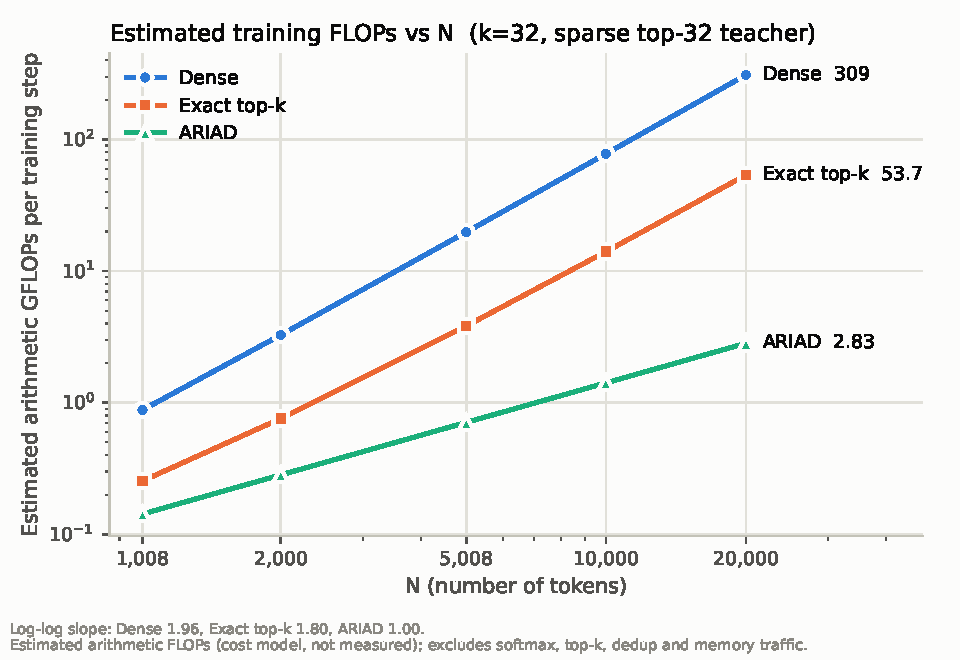
\includegraphics[width=\linewidth]{figures/single_space_cost.pdf}
 \caption{Estimated arithmetic cost per training step ($10^9$ FLOPs) versus $N$, with $k=32$ and $C_{\mathrm{scored}}=144$. The model includes projections, attention, and search; differentiable work is approximated as three forward computations. Softmax, top-$k$, deduplication, gather/scatter, memory traffic, and evaluation audits are excluded. These are cost-model estimates from the seed-0 configurations, not hardware measurements.}
 \label{fig:single-cost}
\end{figure}

\paragraph{Scaling and output quality.}
Table~\ref{tab:single-quality} shows that ARIAD closely approaches Exact top-$k$ at $N=2000$--$10000$: the paired MSE increase is below $2.5\%$ for every seed. At $N=20000$, the mean MSE rises from $0.96$ to $1.11$ ($\times10^{-4}$), a $15.6\%$ increase, and teacher match falls from $0.9767$ to $0.9276$. The fixed search width also yields lower current-graph recall as $N$ grows: its three-seed mean decreases from $0.9953$ at $N=2000$ to $0.9336$ at $N=20000$. Thus, a fixed candidate budget does not preserve retrieval accuracy at every scale. The $N=1008$ runs are still improving at step 500 and should be read as fixed-step results, not asymptotic quality or a reliable ranking of the methods. Dense has higher mean MSE throughout this sweep; this comparison favors sparse students structurally aligned with the sparse teacher and does not establish an unavoidable error floor for dense attention. Approximate neighbors can also change the optimization trajectory, so differences between separately trained Exact and ARIAD students are not solely instantaneous retrieval errors.

The arithmetic savings grow with $N$ (Fig.~\ref{fig:single-cost}). Dense evaluates $N^2$ differentiable pair scores, Exact evaluates $N^2$ search scores plus $Nk$ differentiable scores, and ARIAD evaluates $NC_{\mathrm{scored}}$ search scores plus $Nk$ differentiable scores per step. At $N=20000$, estimated costs are $309.17$, $53.66$, and $2.83$ GFLOPs, respectively; ARIAD uses $5.3\%$ of Exact's estimate. For fixed dimensions, $k$, and $C_{\mathrm{scored}}$, ARIAD's modeled arithmetic is linear in $N$. This does not imply linear end-to-end runtime or a corresponding wall-clock speedup: indexing and memory costs are excluded, and sparse operations may be slower than optimized dense GEMM. Supplementary material gives the cost formula and implementation details.

\begin{figure}[t]
 \centering
 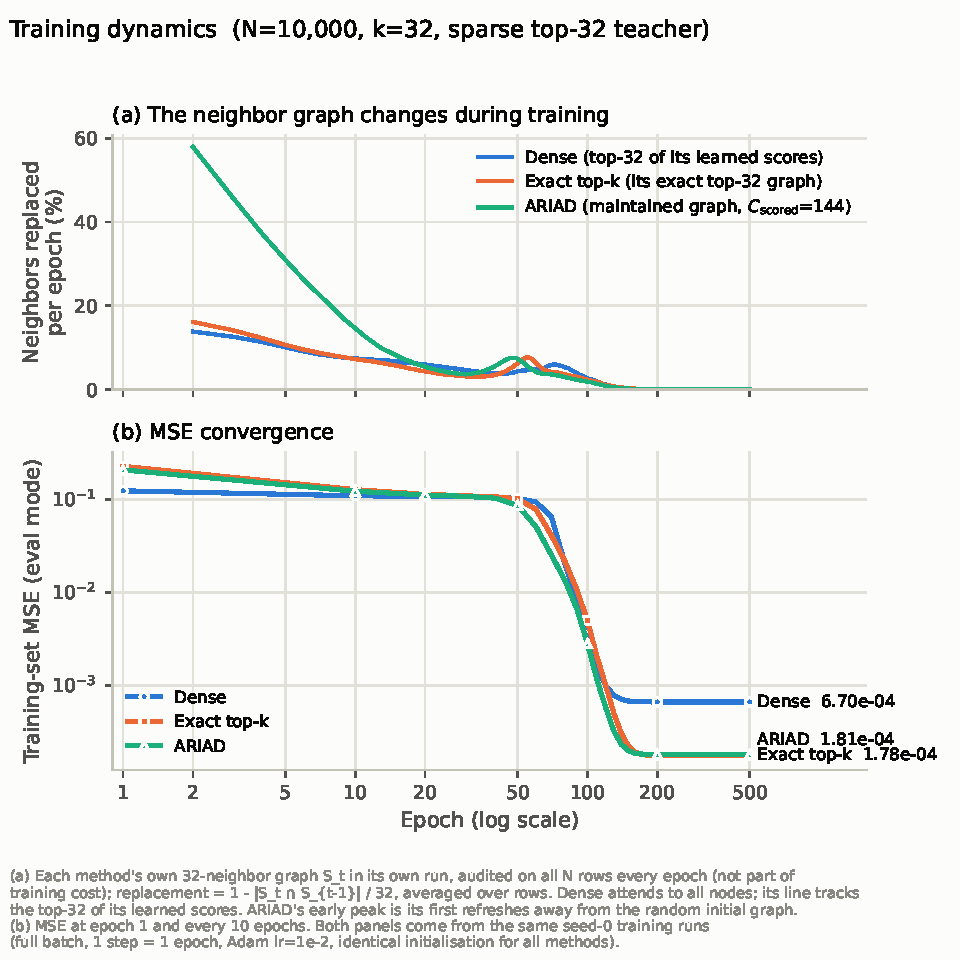
\includegraphics[width=\linewidth]{figures/single_space_training_dynamics.pdf}
 \caption{Training dynamics at $N=10000$, $k=32$, seed 0. (a) Neighbor replacement between consecutive epochs, $100[1-\frac{1}{N}\sum_i |H_t(i)\cap H_{t-1}(i)|/32]$. Each curve uses its own method's training trajectory: Dense's diagnostic top-32 learned scores, Exact's exact top-32 graph, and ARIAD's maintained graph ($C_{\mathrm{scored}}=144$). Dense aggregates over all nonself nodes. These curves do not compare ARIAD with its own current exact graph. (b) Post-update MSE on the training nodes at epoch 1 and every ten epochs, from the same runs. Epochs count optimization steps, not elapsed time. Graph audits cover all rows and are excluded from training costs.}
 \label{fig:single-dynamics}
\end{figure}

\paragraph{Graph evolution and output fitting.}
Figure~\ref{fig:single-dynamics} shows representative seed-0 trajectories at $N=10000$. Panel (a) records substantial neighbor replacement early in training for all three methods, followed by declining turnover as optimization progresses. ARIAD's larger initial replacement reflects its departure from a random neighbor graph. Since the curves describe each method's own trajectory, similar replacement rates do not establish that their neighbor sets agree, nor does low late-stage turnover establish accurate retrieval. Panel (b) complements this graph diagnostic with output MSE: despite its random initial graph, ARIAD reaches $1.815\times10^{-4}$ after 500 steps, close to Exact's $1.779\times10^{-4}$, while Dense reaches $6.70\times10^{-4}$. Together, the panels show that graph updates accompany output fitting throughout training; current-graph recall, reported in the budget analysis below, separately measures retrieval accuracy. This single trajectory does not establish a convergence-rate advantage.

\begin{figure*}[t]
 \centering
 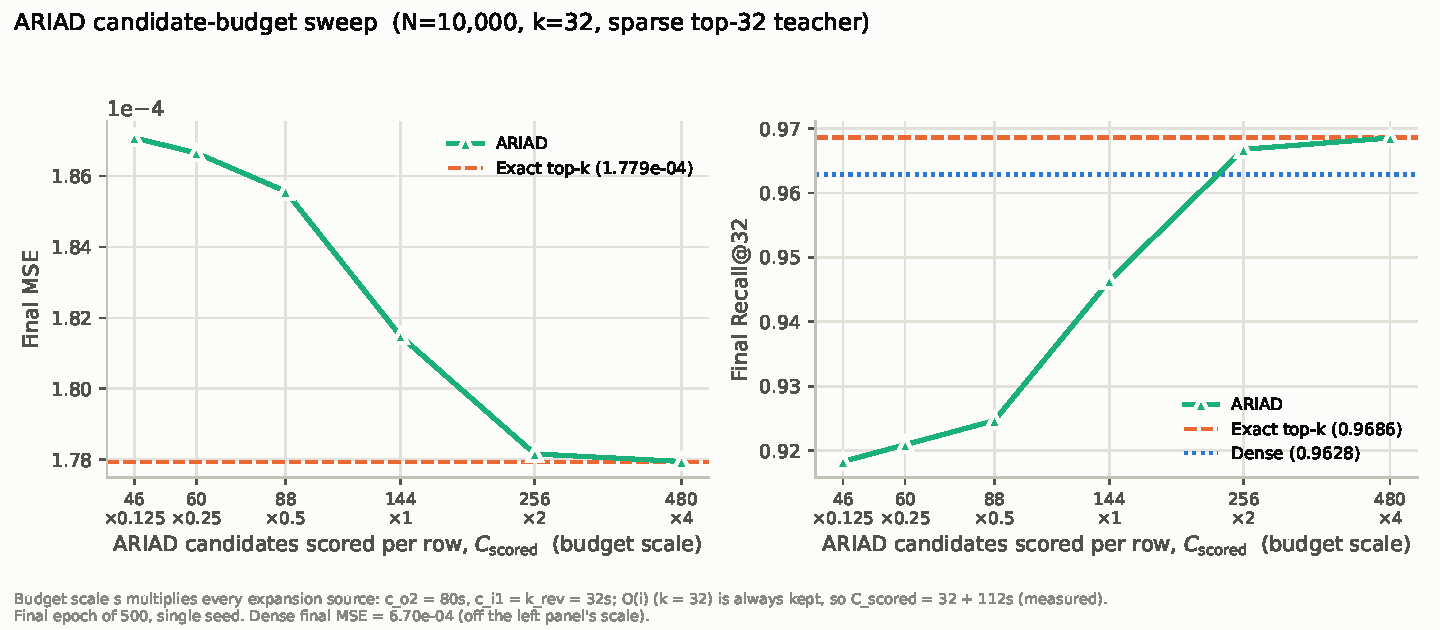
\includegraphics[width=0.92\textwidth]{figures/single_space_budget.pdf}
 \caption{Candidate-budget tradeoff at $N=10000$, $k=32$, after 500 steps (seed 0). Left: MSE on the training nodes. Right: teacher match@32, labeled ``Recall@32'' in the supplied plot; this is distinct from current-graph recall. Expansion budgets scale together, $C_{\mathrm{scored}}=32+112s$, with measured widths $46,60,88,144,256,480$. Dashed lines use the paired Exact top-$k$ reference; the dotted line shows Dense's diagnostic teacher match. Dense's MSE, $6.70\times10^{-4}$, lies outside the left panel's range. The narrow MSE axis makes the approximately $4.9\%$ decrease across the sweep visually prominent.}
 \label{fig:single-budget}
\end{figure*}

\paragraph{Candidate-budget tradeoff.}
In Fig.~\ref{fig:single-budget}, we retain $k=32$ and scale both expansion sources by $s\in\{0.125,0.25,0.5,1,2,4\}$, using $80s$ second-order outgoing candidates and $32s$ incoming-buffer slots; the reverse-buffer capacity also becomes $32s$. Measured $C_{\mathrm{scored}}$ therefore ranges from 46 to 480. Over this range, MSE decreases from $1.871\times10^{-4}$ to $1.780\times10^{-4}$, only about $4.9\%$, while teacher match rises from $0.9183$ to $0.9685$ and current-graph recall rises from $0.9286$ to $0.9996$. Output error is thus less sensitive to the budget than neighbor overlap in this run. At budget 256, MSE is $1.782\times10^{-4}$ versus Exact's $1.779\times10^{-4}$, teacher match is $0.9668$ versus $0.9686$, and current-graph recall is $0.9954$. This uses $2.56\%$ of Exact's search-score count, with estimated cost $1.56$ versus $14.03$ GFLOPs per step. Across all six budgets, ARIAD's estimate ranges from $1.29$ to $1.84$ GFLOPs. These single-seed results characterize the budget tradeoff, without establishing the significance of small MSE differences or resolving the larger-$N$ gap.

Together, these controlled single-space results support online graph maintenance from random neighbors with output quality close to exact top-$k$ attention over much of the sweep and substantially fewer similarity evaluations. They do not establish generalization to natural data, validity in the dual-space setting, or end-to-end runtime acceleration.
